% AWS Lab_2.tex - AWS Lab 2 for Cloud Computing class (Spring 2015)
% Chanmann Lim - March 2015

\documentclass[a4paper]{article}

\usepackage[margin=1 in]{geometry}
\usepackage{listings}
\usepackage{graphicx}
\usepackage{float}

\begin{document}
\title{CS 7001-03: Report for AWS Lab 2 - AWS Resource Discovery and Instance Setup}
\author{Chanmann Lim\\ 
	\texttt{cl9p8@mail.mail.missouri.edu}}
\date{March 03, 2015}
\maketitle


Install \texttt{awscli} tool via easy\_install \texttt{pip} on Mac OS.

% ---------------------------------------- 1 ----------------------------------------
\paragraph{1. } Create an AWS key pair using \texttt{aws ec2 create-key-pair} command with \texttt{--key-name} option set to 'cloud-key':
\begin{verbatim}
# aws ec2 create-key-pair --key-name cloud-key
\end{verbatim}

Delete a key pair using \texttt{aws ec2 delete-key-pair} command with \texttt{--key-name} option set to 'cloud-key':
\begin{verbatim}
# aws ec2 delete-key-pair --key-name cloud-key
\end{verbatim}

% ---------------------------------------- 2 ----------------------------------------
\paragraph{2. } Create a security group in AWS. \\

Use \texttt{aws ec2 create-security-group} command with options
\begin{description}
\leftskip 0.4in
\parindent -0.4in
	\item[\texttt{--group-name} : ] set security group name.
	\item[\texttt{--description} : ] set security group description.
\end{description}

and adding inbound traffic rule to security group via \texttt{aws ec2 authorize-security-group-ingress} command with options
\begin{description}
\leftskip 0.4in
\parindent -0.4in
	\item[\texttt{--group-name} : ] security group name.
	\item[\texttt{--protocol} : ] IP protocol eg. tcp, udp or icmp.
	\item[\texttt{--port} : ] tcp or tcp port range.
	\item[\texttt{-cidr} : ] IP range.
\end{description}
\begin{verbatim}
# aws ec2 create-security-group  \
      --group-name cloud-group   \
      --description "Open ports"
# aws ec2 authorize-security-group-ingress \
      --group-name cloud-group             \
      --protocol tcp                       \
      --port 22                            \
      --cidr 0.0.0.0/0
# aws ec2 authorize-security-group-ingress \
      --group-name cloud-group             \
      --protocol tcp                       \
      --port 80                            \
      --cidr 0.0.0.0/0
# aws ec2 authorize-security-group-ingress \
      --group-name cloud-group             \
      --protocol tcp                       \
      --port 443                            \
      --cidr 0.0.0.0/0
\end{verbatim}

Delete security group via \texttt{aws ec2 delete-security-group} command with \texttt{--group-name} option set to 'cloud-group'.

\begin{verbatim}
# aws ec2 delete-security-group --group-name cloud-group
\end{verbatim}

% ---------------------------------------- 3 ----------------------------------------
\paragraph{3. } Execute command:
\begin{verbatim}
# aws ec2 run-instances --image-id ami-caf9a6a2 \
--instance-type t1.micro \
--count 2 \
--key-name cloud-key \
--security-groups cloud-group \
--region us-east-1
\end{verbatim}
will result in launching two instances (servers) in North Virginia(us-east-1) Amazon cloud using private Amazon Machine Image (AMI) --  "ami-caf9a6a2" as the template, configuring security group to "cloud-group" (SSH, HTTP and HTTPS are opened) and embedding "cloud-key" key pair for ssh login to both instances without password. \\

Terminate the instances, delete "cloud-key" key pair and "cloud-group" security group with following commands: 
\begin{verbatim}
# aws ec2 terminate-instances --instance-ids i-09925ef9 i-f5935f05
# aws ec2 delete-key-pair --key-name cloud-key
# aws ec2 delete-security-group --group-name cloud-group
\end{verbatim}
\begin{figure}[H]
  \centering
    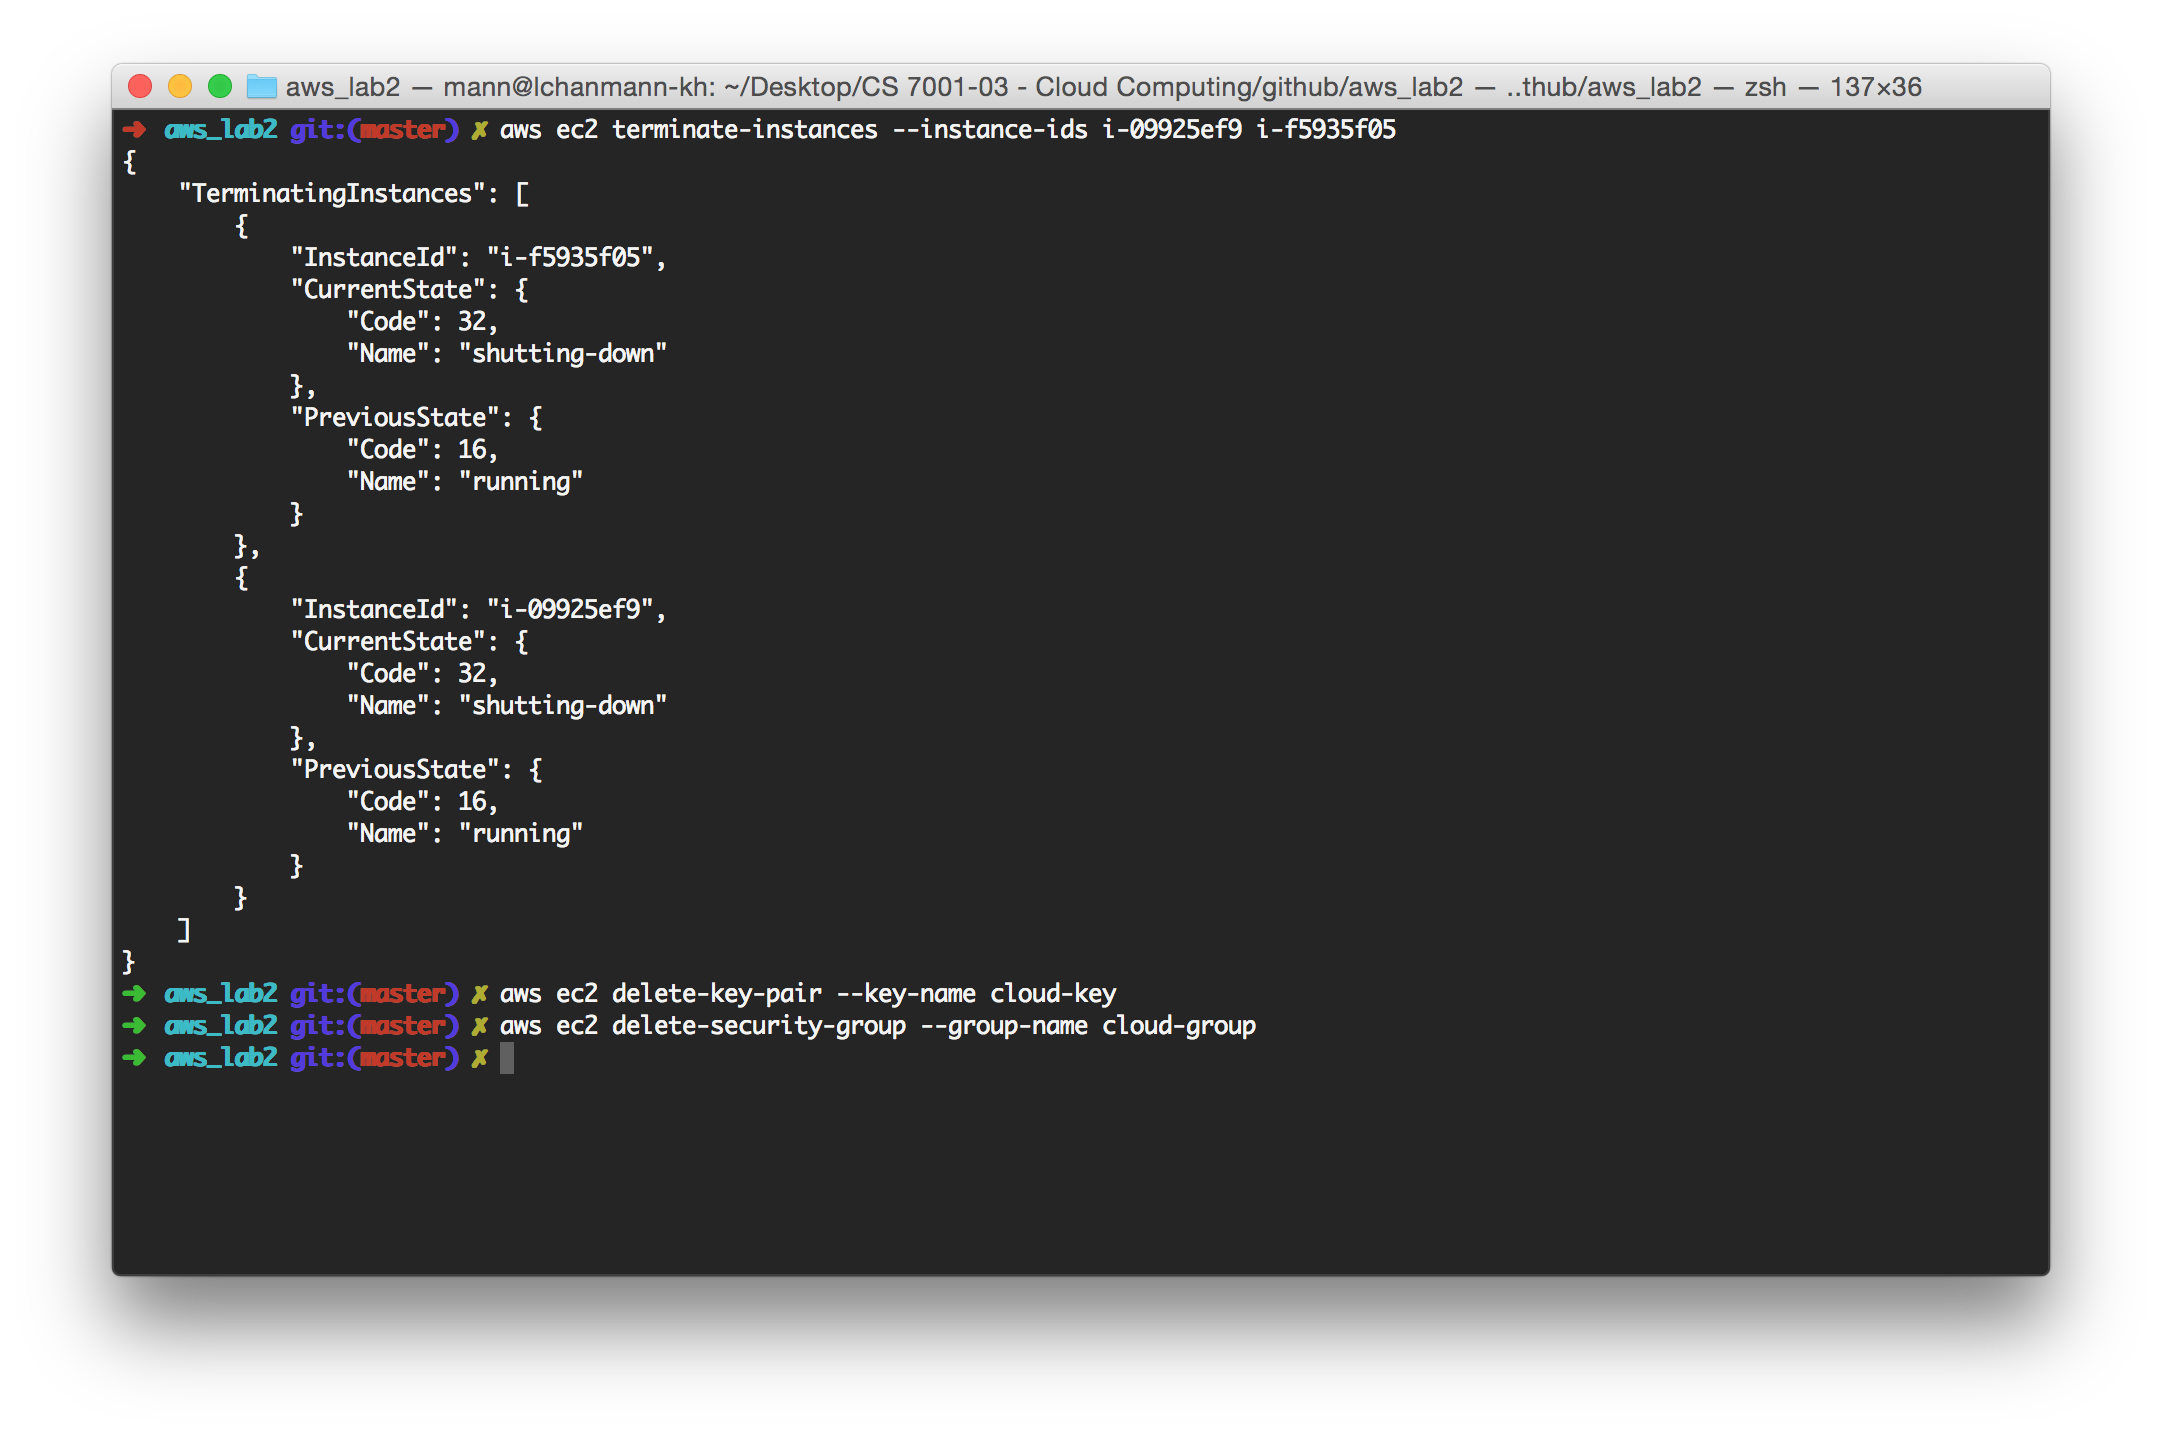
\includegraphics[scale=.4]{terminate_instances.png}
  \caption{Terminate instances, delete key pair and security group.}
\end{figure}

% ---------------------------------------- 4 ----------------------------------------
\paragraph{4. } Get status information of all instances using aws-cli commands.
\begin{verbatim}
# aws ec2 describe-instance-status
\end{verbatim}
\begin{figure}[H]
  \centering
    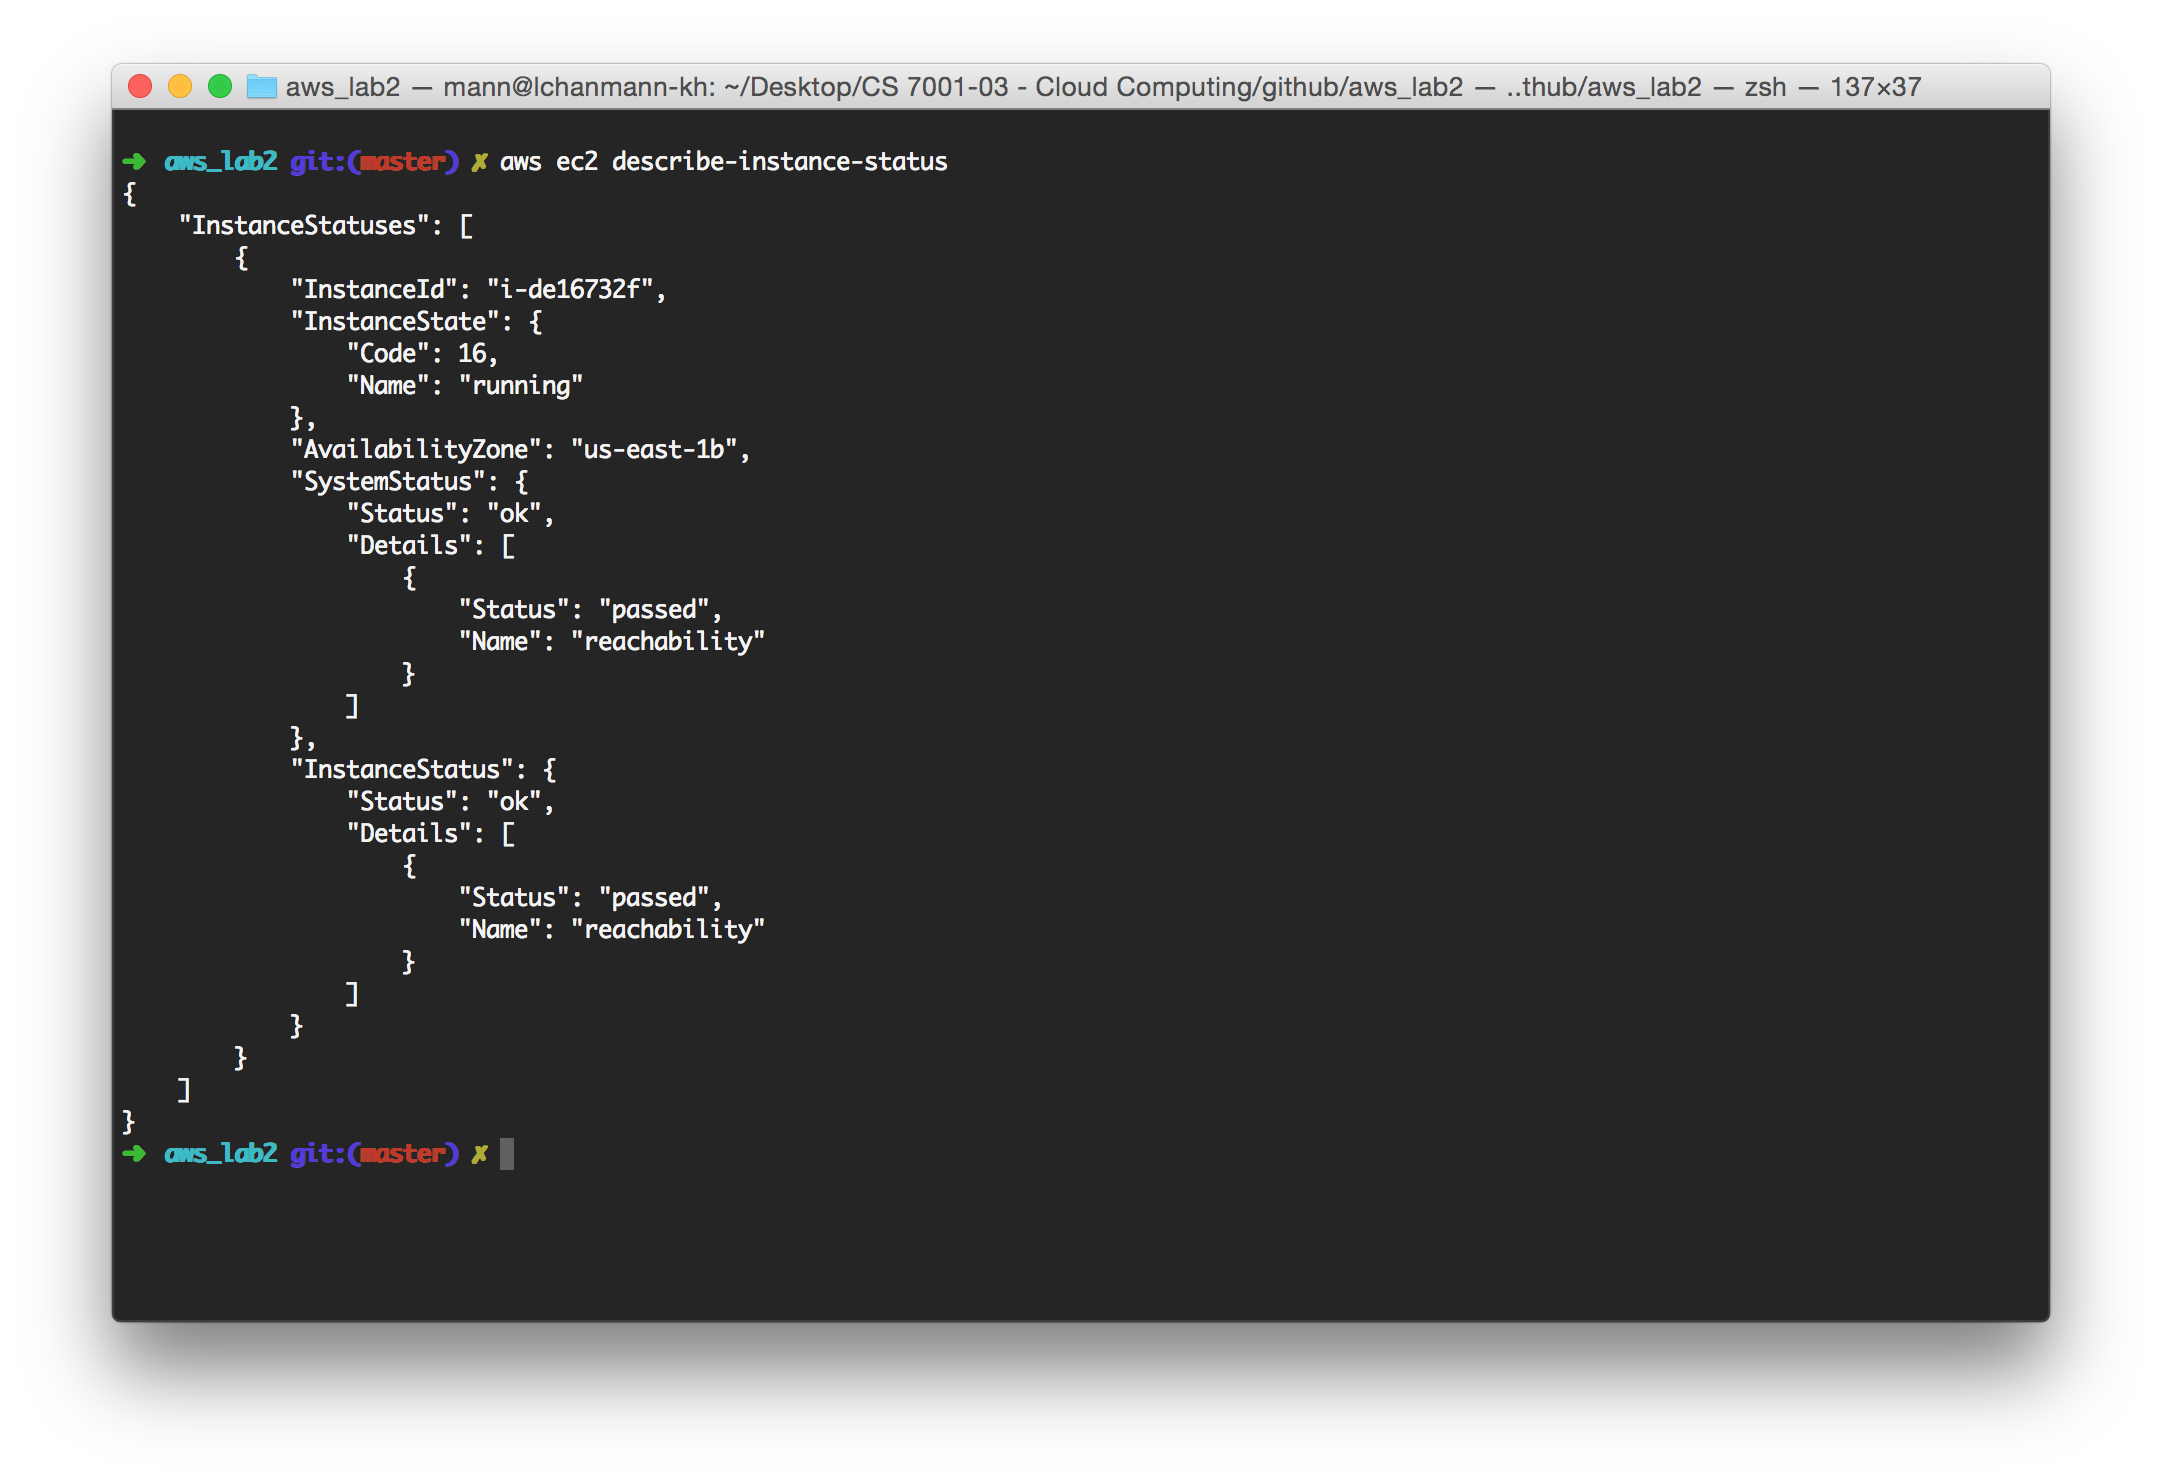
\includegraphics[scale=.4]{instance_status.png}
  \caption{AWS instances status}
\end{figure}

% ---------------------------------------- 5 ----------------------------------------
\paragraph{5. } Create snapshot command: \texttt{aws ec2 create-snapshot} with options
\begin{description}
\leftskip 0.4in
\parindent -0.4in
	\item[\texttt{--volume-id} : ] set EBS volume to be snapshot.
	\item[\texttt{--description} : ] set snapshot description.
\end{description}
\begin{verbatim}
# aws ec2 create-snapshot      \
      --volume-id vol-54c4644f \
      --description "Backup"
\end{verbatim}

Delete snapshot command: \texttt{aws ec2 delete-snapshot} with \texttt{--snapshot-id} option.
\begin{verbatim}
# aws ec2 delete-snapshot --snapshot-id snap-51cf8cd0
\end{verbatim}


% ---------------------------------------- 6 ----------------------------------------
\paragraph{6. } Add a new EBS volume with \texttt{aws ec2 create-volume} with options:
\begin{description}
\leftskip 0.4in
\parindent -0.4in
	\item[\texttt{--size} : ] set volume size (in GB).
	\item[\texttt{--availability-zone} : ] set availability zone of the volume.
\end{description}
\begin{verbatim}
#aws ec2 create-volume --size 3 --availability-zone us-east-1b
\end{verbatim}

Attach the volume to the running instance (i-de16732f) via \texttt{aws ec2 attach-volume} with options:
\begin{description}
\leftskip 0.4in
\parindent -0.4in
	\item[\texttt{--volume-id} : ] set volume id to attach.
	\item[\texttt{--instance-id} : ] set instance id to be attached to.
	\item[\texttt{--device} : ] set device name with which the instance will use to interact.
\end{description}
\begin{verbatim}
#aws ec2 attach-volume        \
     --volume-id vol-3ae79321 \
     --instance-id i-de16732f \
     --device /dev/sdh
\end{verbatim}
\begin{figure}[H]
  \centering
    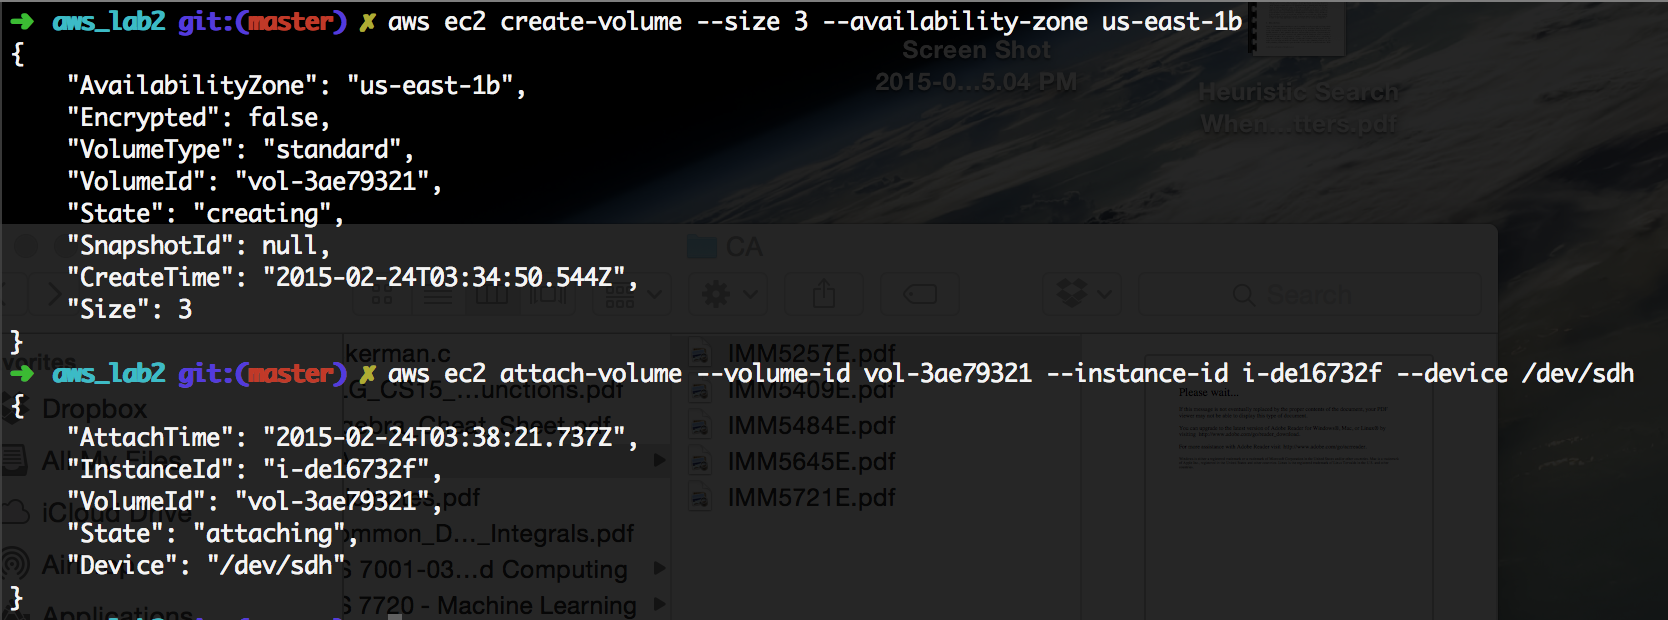
\includegraphics[scale=.4]{attaching_volume.png}
  \caption{Create and attach volume using aws-cli}
\end{figure} 
\begin{figure}[H]
  \centering
    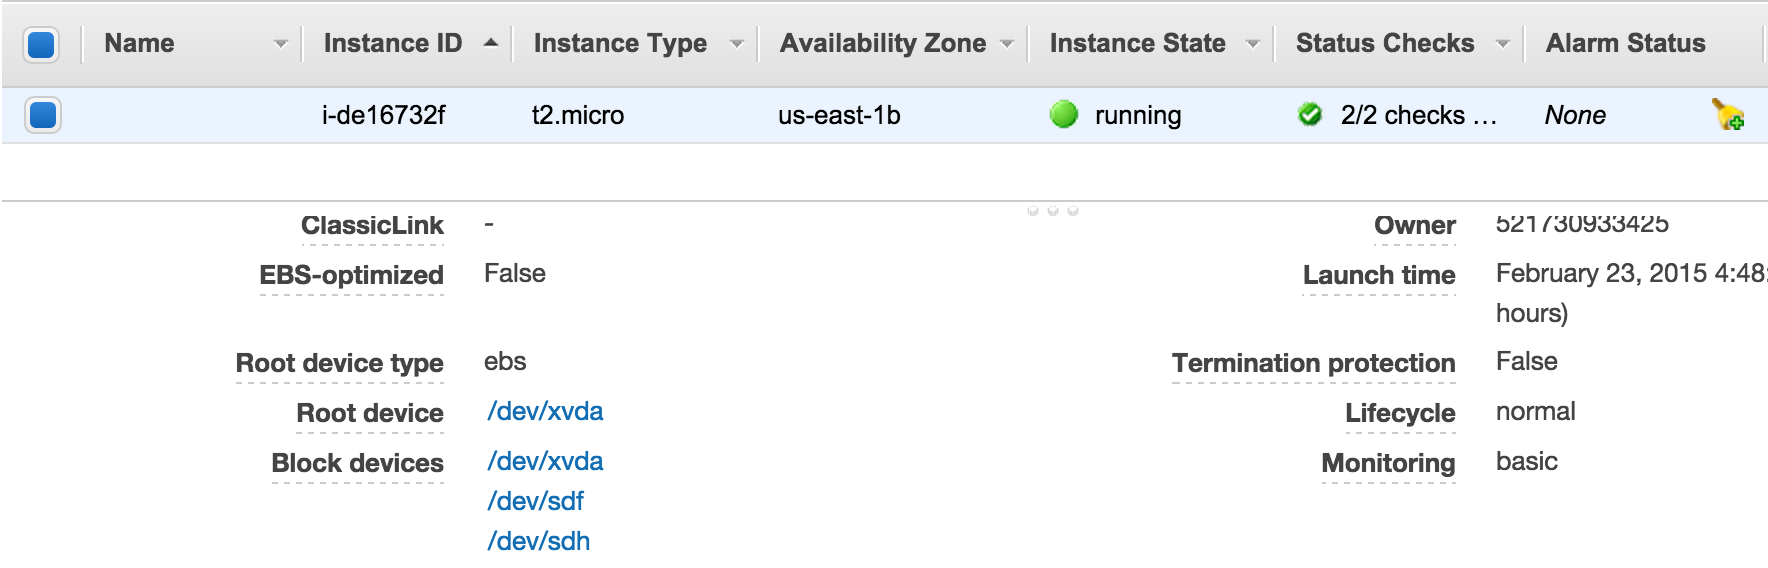
\includegraphics[scale=.4]{attached_volume.png}
  \caption{The new volume is attached to /dev/sdh}
\end{figure} 

% ---------------------------------------- 7 ----------------------------------------
\paragraph{7. } Provide a screenshot taken in Step 3.4.2 \\

\texttt{http://ec2-52-1-133-200.compute-1.amazonaws.com/} \\
\begin{figure}[H]
  \centering
    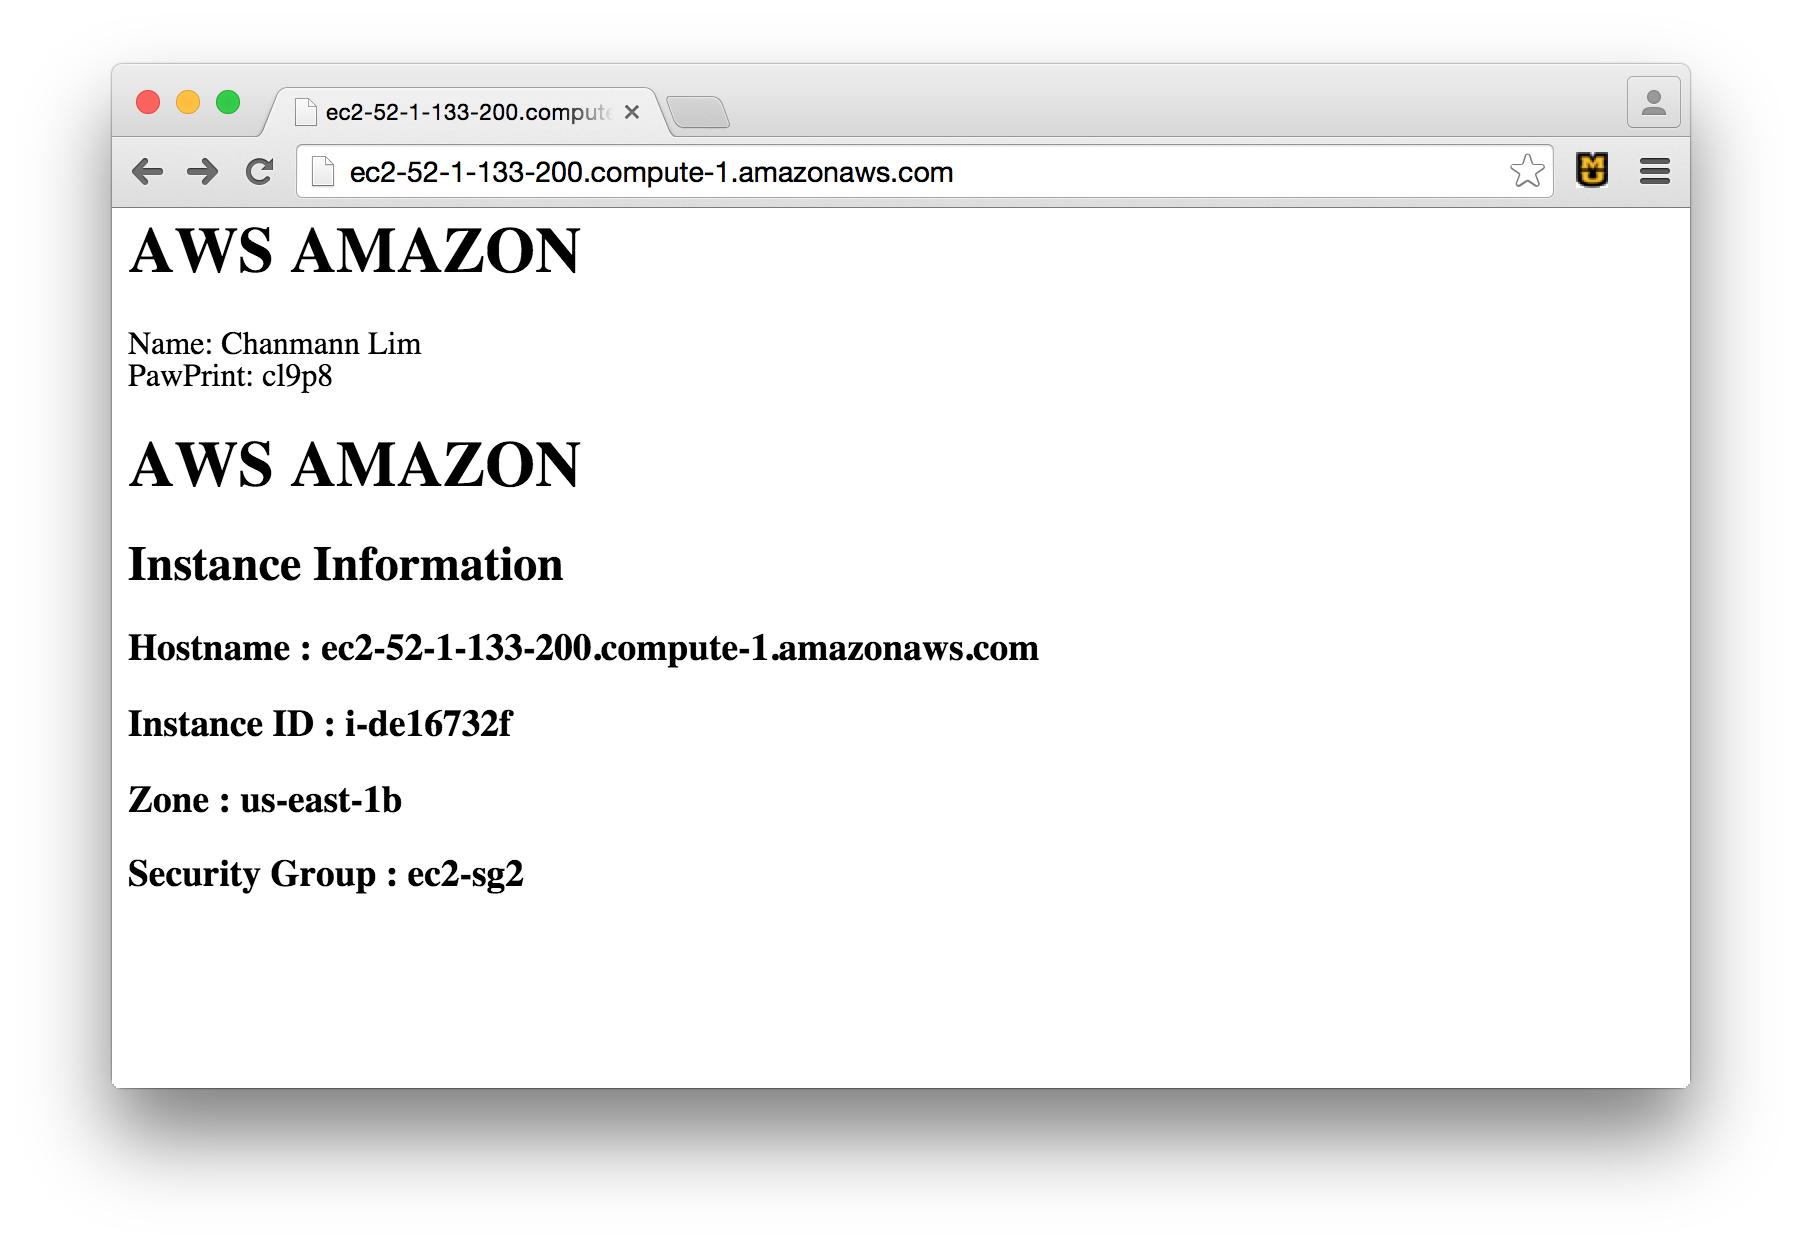
\includegraphics[scale=.4]{aws_web_server.png}
  \caption{AWS web server}
\end{figure} 

% ---------------------------------------- 8 ----------------------------------------
\paragraph{8. } The six best practices described by Amazon AWS:
\begin{description}
\leftskip 0.4in
\parindent -0.4in
	\item[Design for failure and nothing will fail : ] \hfill \\ By assuming everything can fail (hardware failure, software failure, outage and failure due to natural disaster), application architects should embrace automated recovery for data, OS configurations, and in-progress jobs processing.
	\item[Decouple your components : ] \hfill \\ The cloud encourages Service-Oriented-Architecture for decoupling the components in the system to support concurrency, high availability.
	\item[Implement elasticity : ] \hfill \\ Automated scaling by automating deployment process with script to help reduce error and facilitate an efficient and scalable update process.
	\item[Think parallel : ] \hfill \\ The cloud architects should parallelize their applications to make them thread-safe, multi-threading and request parallelization to achieve maximum performance and throughput.
	\item[Keep dynamic data closer to the compute and static data closer to the end-user : ] \hfill \\ To reduce the processing and internet latency by moving the data and data-consuming applications into the cloud and moving static content such as images, videos, audios, pdfs, etc., into content delivery network which get cached at edge locations closer to the users to lower the access latency.
	\item[Security Best Practices: ] \hfill \\ Developers should implement security best practices and standard methods such as 1) configuring SSL or setting up Virtual Private Cloud for sensitive information exchanges, 2) using file encryption tools to secure the storage, 3) using AWS access key and access key rotation when the key get compromised or X.509 certificates for authentication and multi-factor authentication with Amazon account information, 3) using AWS Identity and Access Management (IAM) to manage user permission on accessing AWS services, 4) configuring security group for incoming network traffic, using firewall softwares (\emph{netfilter} and \emph{iptables}), regularly updating patches and run security checks.
\end{description}
\end{document}